\subsection{What Research is the Storage used for?}

\begin{frame}[c]{Why Classify Storage Usage?}
    \noindent
    \begin{minipage}[c]{0.6\linewidth}
        \large
        \begin{itemize}[<+(1)->]
            \item Financial backers want to know what they pay for
            \begin{itemize}[<+(1)->]
                \item Ministery for Science, Research and Culture (MWK BW)
                \item KIT
                \item Helmholtz-Society
            \end{itemize}
            \item Particularly if it is used well%, and what for
            \item Good existing classification from 'Deutsche~Forschungsgesellschaft'
        \end{itemize}
    \end{minipage} % no space if you would like to put them side by side
    \begin{minipage}[c]{0.3\linewidth}
    % 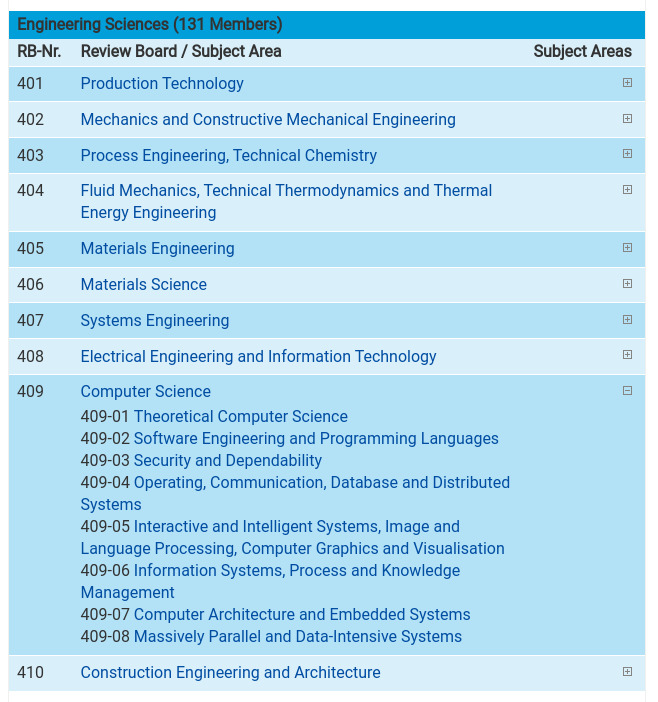
\includegraphics[width=\textwidth,right]{Selection_032} \\
        \pause
    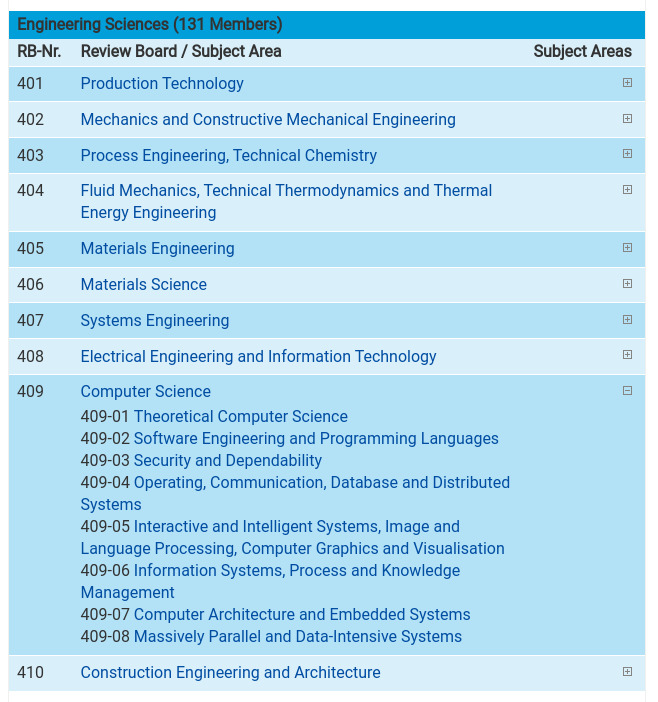
\includegraphics[height=0.85\textheight]{Selection_032} \\
        % \begin{itemize}[<+(1)->]
        %     \item Some other text here
        % \end{itemize}
    \end{minipage}
    % 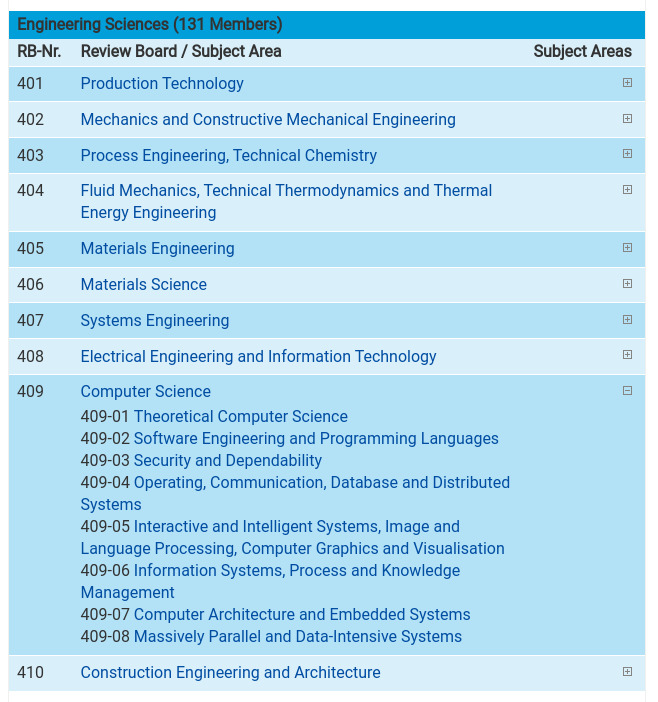
\includegraphics[width=0.4\textwidth,right]{Selection_032} \\
\end{frame}

% \begin{frame}[c]{Why Classify Storage Usage? Orig}
%     \begin{multicols}{2}
%         \begin{itemize}[<+(1)->]
%             \item Financial backers want to know what their money is being spent on
%             \begin{itemize}[<+(1)->]
%                 \item Ministery for Science, Research and Culture (MWK BW)
%                 \item KIT
%                 \item Helmholtz-Society
%             \end{itemize}
%             \item Particularly if it is used well, and what for
%             \item Good existing classification from 'Deutsche~Forschungsgesellschaft'
%         \end{itemize}
%         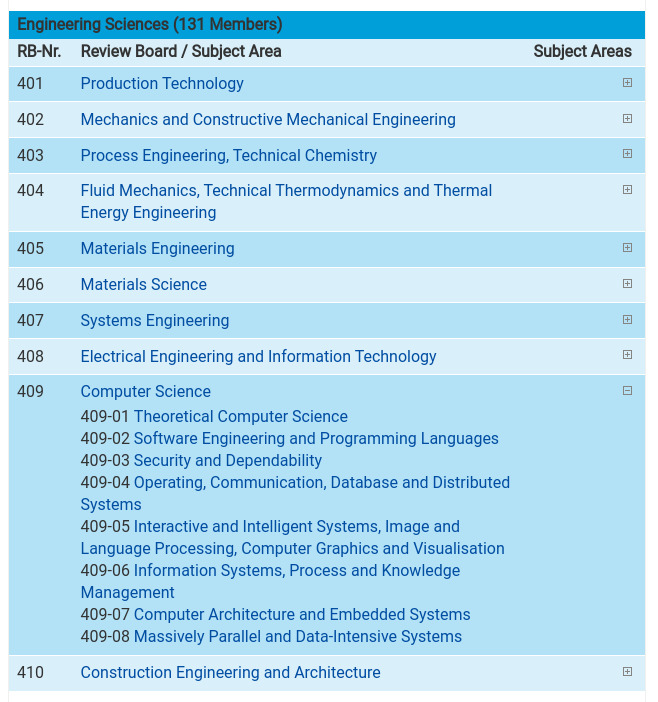
\includegraphics[width=0.45\textwidth,right]{Selection_032} \\
%     \end{multicols}
% \end{frame}

\pic{Selection of DFG Subject Area upon Project Creation}{10}

% \begin{frame}[c]{Selection of DFG Discipline}
%     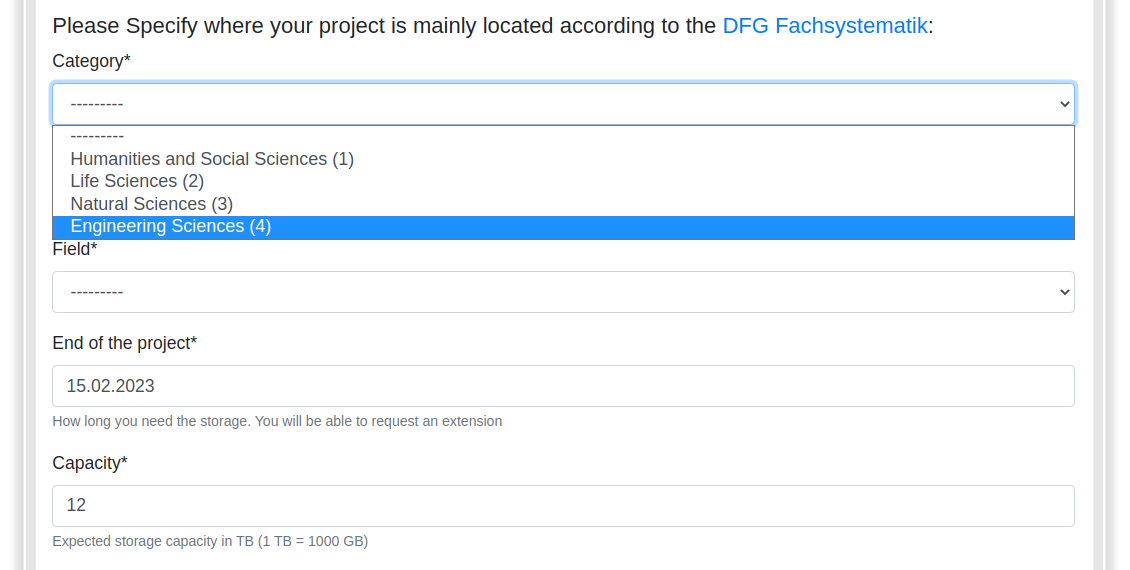
\includegraphics[width=\textwidth]{select_category}
% \end{frame}
% \begin{frame}[c]{Selection of DFG Subject Area without Board}
%     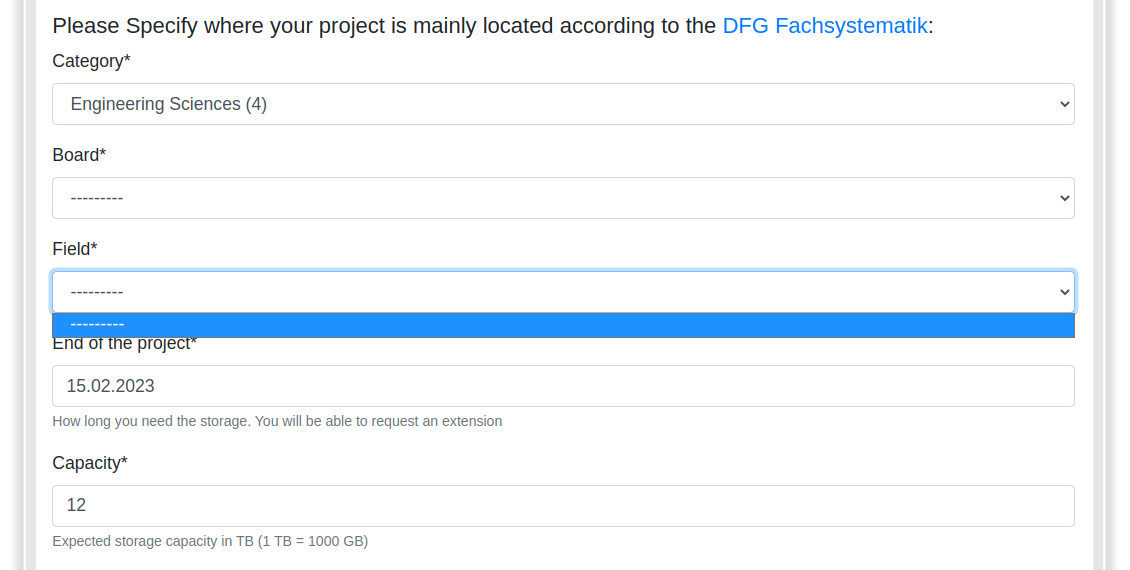
\includegraphics[width=\textwidth]{select_field1}
% \end{frame}
% \begin{frame}[c]{Selection of DFG Review Board}
%     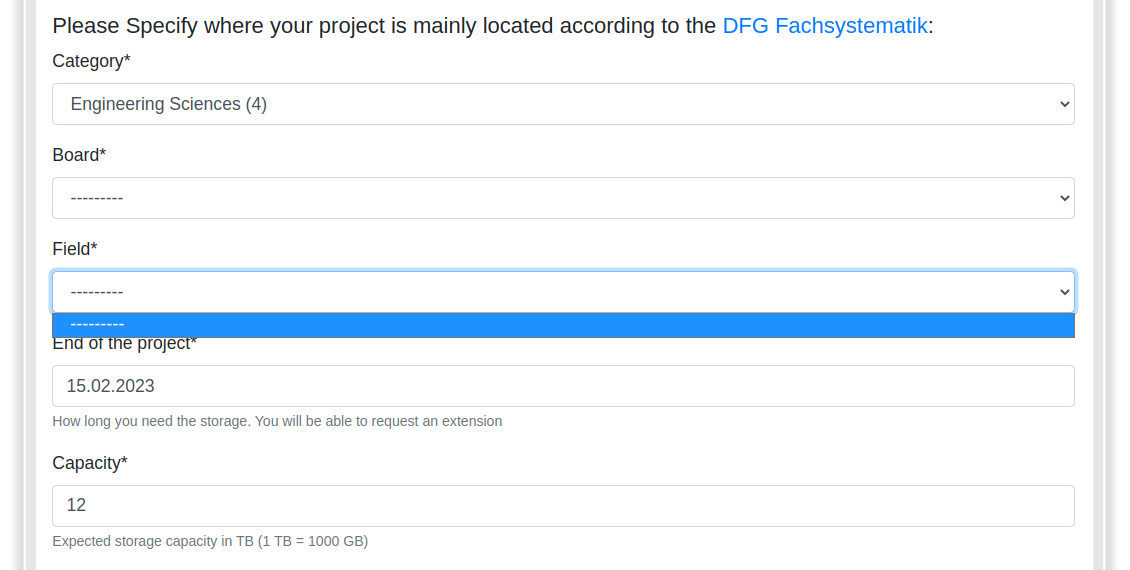
\includegraphics[width=\textwidth]{select_field1}
% \end{frame}
% \begin{frame}[c]{Selection of DFG Subject Area}
%     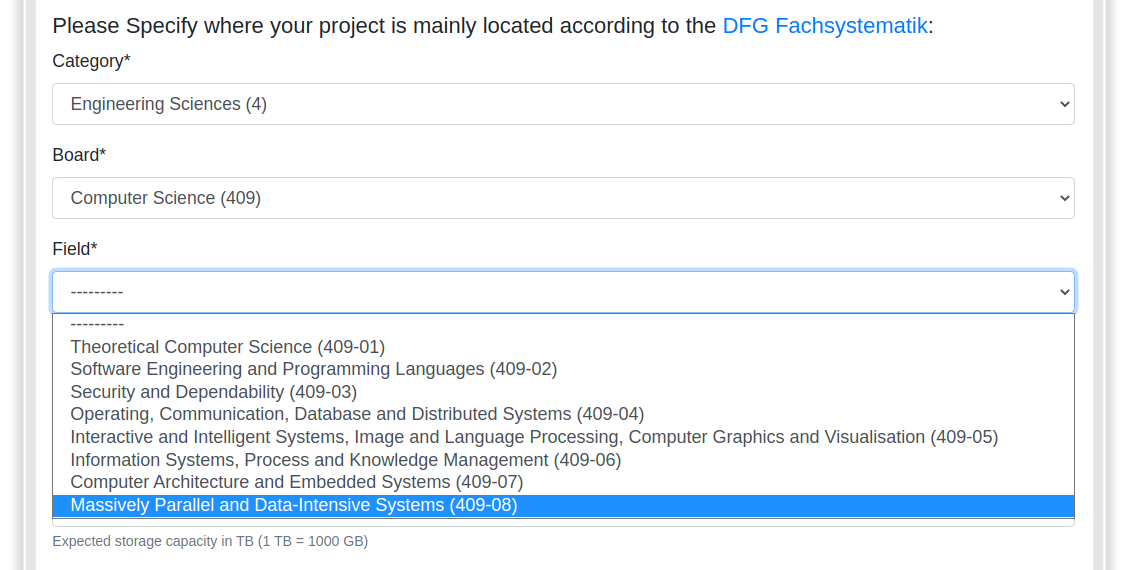
\includegraphics[width=\textwidth]{select_field2}
% \end{frame}


\begin{frame}[c]{Request Visualisation}
    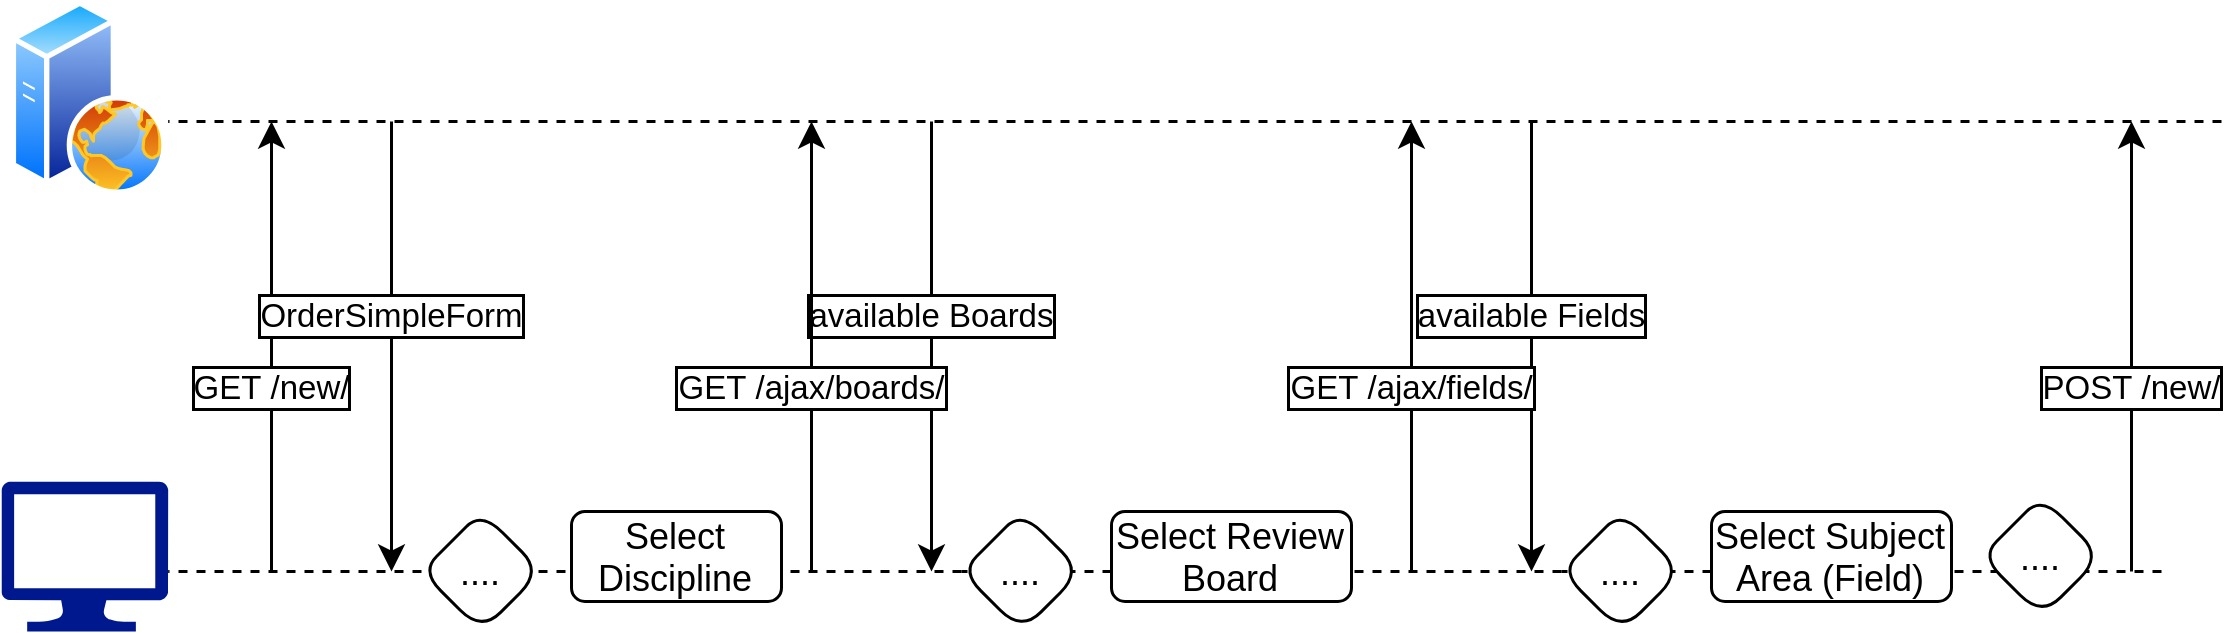
\includegraphics[width=\textwidth]{board_requests}
\end{frame}

\begin{frame}[c,fragile]{Webpage: Requesting Fields for Boards}
    \footnotesize
    \inputminted[linenos=true]{javascript}{code/board_request.js}
\end{frame}

\begin{frame}[c,fragile]{Backend: Answering With Available Fields}
\footnotesize
    \begin{minted}[linenos]{python}
## urls.py      # path(route: str, view: callable, name: str)
path(route='ajax/fields/', view=view_science_fields, name="ajax_load_fields")

## views.py
def view_science_fields(request: HTTPRequest):
    b_pk = request.GET.get('board')  # we get the pk of the selected board
    if b_pk:  # select the Fields that are members of this Board
        fields = Science_Field.objects.filter(board__pk=b_pk) 
        # SELECT field WHERE field.board.pk == b_pk
        return render(request, 'dropdown_list_options.html',
                      {'dropodwn_items': fields}
                    )
    return render(request, 'dropdown_list_options.html',
                  {'dropodwn_items': Science_Field.objects.none()}
                )
\end{minted}
\end{frame}

